%%%%%%%%%%%%%%%%%%%%%%%%%%%%%%%%%%%%%%%%%
% University Assignment Title Page 
% LaTeX Template
% Version 1.0 (27/12/12)
%
% This template has been downloaded from:
% http://www.LaTeXTemplates.com
%
% Original author:
% WikiBooks (http://en.wikibooks.org/wiki/LaTeX/Title_Creation)
%
% License:
% CC BY-NC-SA 3.0 (http://creativecommons.org/licenses/by-nc-sa/3.0/)
% 
% Instructions for using this template:
% This title page is capable of being compiled as is. This is not useful for 
% including it in another document. To do this, you have two options: 
%
% 1) Copy/paste everything between \begin{document} and \end{document} 
% starting at \begin{titlepage} and paste this into another LaTeX file where you 
% want your title page.
% OR
% 2) Remove everything outside the \begin{titlepage} and \end{titlepage} and 
% move this file to the same directory as the LaTeX file you wish to add it to. 
% Then add \input{./title_page_1.tex} to your LaTeX file where you want your
% title page.
%
%%%%%%%%%%%%%%%%%%%%%%%%%%%%%%%%%%%%%%%%%
%\title{Title page with logo}
%----------------------------------------------------------------------------------------
%	PACKAGES AND OTHER DOCUMENT CONFIGURATIONS
%----------------------------------------------------------------------------------------

\documentclass[12pt]{article}
\usepackage[english]{babel}
\usepackage[utf8x]{inputenc}
\usepackage{amsmath}
\usepackage{graphicx}
\usepackage[colorinlistoftodos]{todonotes}

\begin{document}

\begin{titlepage}

\newcommand{\HRule}{\rule{\linewidth}{0.5mm}} % Defines a new command for the horizontal lines, change thickness here

\center % Center everything on the page
 
%----------------------------------------------------------------------------------------
%	HEADING SECTIONS
%----------------------------------------------------------------------------------------

\textsc{\LARGE The University of Sydney}\\[1.5cm] % Name of your university/college
\textsc{\Large School of Information Technology}\\[0.5cm] % Major heading such as course name
\textsc{\large INFO5993 Research Methods - Assignment I}\\[0.5cm] % Minor heading such as course title

%----------------------------------------------------------------------------------------
%	TITLE SECTION
%----------------------------------------------------------------------------------------

\HRule \\[0.4cm]
{ \huge \bfseries Report on Database Searching Result, Annotated Bibliography, Proposing methodologies}\\[0.4cm] % Title of your document
\HRule \\[1.5cm]
 
%----------------------------------------------------------------------------------------
%	AUTHOR SECTION
%----------------------------------------------------------------------------------------

\begin{minipage}{0.4\textwidth}
\begin{flushleft} \large
\emph{Author:}\\
Lin \textsc{Han} % Your name
\end{flushleft}
\end{minipage}
~
\begin{minipage}{0.4\textwidth}
\begin{flushright} \large
\emph{Supervisor:} \\
Dr. Vincent \textsc{Gramoli} % Supervisor's Name
\end{flushright}
\end{minipage}\\[2cm]

% If you don't want a supervisor, uncomment the two lines below and remove the section above
%\Large \emph{Author:}\\
%John \textsc{Smith}\\[3cm] % Your name

%----------------------------------------------------------------------------------------
%	DATE SECTION
%----------------------------------------------------------------------------------------

{\large \today}\\[2cm] % Date, change the \today to a set date if you want to be precise

%----------------------------------------------------------------------------------------
%	LOGO SECTION
%----------------------------------------------------------------------------------------


\includegraphics{logo.png}\\[1cm] % Include a department/university logo - this will require the graphicx package
 
%----------------------------------------------------------------------------------------

\vfill % Fill the rest of the page with whitespace

\end{titlepage}


% \begin{abstract}
% Your abstract.
% \end{abstract}

\section{Introduction}

Blockchain is the one of the most cutting edge technologies in the world nowadays. Not limited to digital currencies like Bitcoin, Etherum, and etc., blockchain enables innovations in wide range of fields, such as distributed cloud storage, digital identity, and smart contracts.
\newline
\newline
This report is trying to give a overview of the research base about blockchain and zero knowledge contingent proof, namely famous conferences and journals, research groups and people. Also, a list of possible unaddressed problems will be given to show possible research directions for my research project. In addition, five core articles or books in this area will be identified along with their annotated bibliography. At the end of this report, a summary of potential research methods will be given on the addressed questions.

\section{Research Base}
\label{sec:research base}

\subsection{List of A*, A Conferences and Journals}
A* conferences and journals:
\begin{enumerate}
\item ACM Symposium on Principles of Distributed Computing - PODC
\item ACM Symposium on Operating Systems Principles - SOSP
\item IEEE Transactions on Parallel and Distributed Systems - TPDS
\end{enumerate}
A conferences and journals:
\begin{enumerate}
\item IEEE International Symposium on Network Computing and Applications - NCA
\item EuroSys
\item IEEE/IFIP International Conference on Dependable Systems - DSN
\end{enumerate}

\subsection{Research Groups}

\begin{enumerate}
\item Initiative for Cryptocurrency and Contracts (IC3) 
\item University of Sydney Concurrent Systems Research Group
\item Cornell University Systems and Networking Research Group
\end{enumerate}

\section{Research Problems}
\label{sec:research problems}

Based on the research and the current progress of RedBelly Blockchain by CSRG, there are three potential problems identified to research which can enrich current RedBelly Blockchain:

\begin{enumerate}
\item Is it possible to make use of an existing zero knowledge proof library in a blockchain system that does not require delay between block creation?
\item Is it possible to constraint the library in the number of participants to which messages should be broadcast so that the transaction remains consistent?
\item Is it possible to make the content of a transaction private (by using for example public key cryptosystems) so that only the payer and the payee can benefit from the transaction?
\end{enumerate}
The above three problems mainly focuses on the zero knowledge contingent proof in blockchain, in detail, the possibility of its integration with RedBelly Blockchain and mobile devices.

\section{Core Articles and Books}
\label{sec:core articles and books}

\subsection{Efficient Zero-Knowledge Contingent Payments in Cryptocurrencies Without Scripts\cite{Banasik2016}}

\subsection{On the Danger of Private Blockchains\cite{Gra16}}

\subsection{The Balance Attack or Why Forkable Blockchains Are Ill-Suited for Consortium\cite{NG17}}

\subsection{The Blockchain Anomaly\cite{NG16}}

\subsection{(Leader/Randomization/Signature)-free Byzantine Consensus for Consortium Blockchains\cite{DBLP:journals/corr/CrainGLR17}}

\subsection{Zerocash: Decentralized anonymous payments from bitcoin\cite{sasson2014zerocash}}

\subsection{The electronic cash system based on non-interactive zero-knowledge proofs\cite{doi:10.1080/00207160.2014.933816}}

\subsection{Succinct non-interactive zero-knowledge proofs with preprocessing for LOGSNP\cite{kalai2006succinct}}

\subsection{Secure Sampling of Public Parameters for Succinct Zero Knowledge Proofs\cite{ben2015secure}}

\subsection{Zero Knowledge Contingent Payment\cite{wiki2011zero}}

% \todo[inline, color=green!40]{This is an inline comment.}

% \subsection{Tables and Figures}

% Use the table and tabular commands for basic tables --- see Table~\ref{tab:widgets}, for example. You can upload a figure (JPEG, PNG or PDF) using the files menu. To include it in your document, use the includegraphics command as in the code for Figure~\ref{fig:frog} below.

% % Commands to include a figure:
% \begin{figure}
% \centering
% 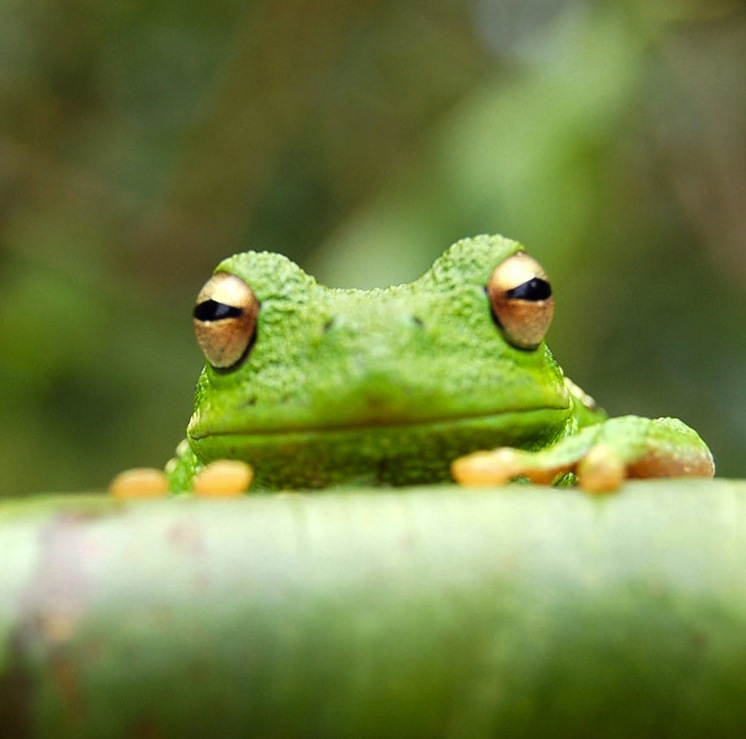
\includegraphics[width=0.5\textwidth]{frog.jpg}
% \caption{\label{fig:frog}This is a figure caption.}
% \end{figure}

% \begin{table}
% \centering
% \begin{tabular}{l|r}
% Item & Quantity \\\hline
% Widgets & 42 \\
% Gadgets & 13
% \end{tabular}
% \caption{\label{tab:widgets}An example table.}
% \end{table}

% \subsection{Mathematics}

% \LaTeX{} is great at typesetting mathematics. Let $X_1, X_2, \ldots, X_n$ be a sequence of independent and identically distributed random variables with $\text{E}[X_i] = \mu$ and $\text{Var}[X_i] = \sigma^2 < \infty$, and let
% $$S_n = \frac{X_1 + X_2 + \cdots + X_n}{n}
%       = \frac{1}{n}\sum_{i}^{n} X_i$$
% denote their mean. Then as $n$ approaches infinity, the random variables $\sqrt{n}(S_n - \mu)$ converge in distribution to a normal $\mathcal{N}(0, \sigma^2)$.

% \subsection{Lists}

% You can make lists with automatic numbering \dots

% \begin{enumerate}
% \item Like this,
% \item and like this.
% \end{enumerate}
% \dots or bullet points \dots
% \begin{itemize}
% \item Like this,
% \item and like this.
% \end{itemize}

% We hope you find write\LaTeX\ useful, and please let us know if you have any feedback using the help menu above.

\newpage
\bibliography{bibliography.bib}
\bibliographystyle{plain}

\end{document}